% !TeX root = ../../Skript.tex
\cohead{\Large\textbf{Punktprobe}}
\fakesubsection{Punktprobe}
Ein besserer Begriff für Punktprobe wäre Punkteinsetzen. Sind eine Funktion \(f(x)\) und ein Punkt \(P(x_P\vert y_P)\) gegeben, so kann man prüfen, ob das Schaubild von \(f(x)\) durch den Punkt verläuft, indem man den Punkt einsetzt:
\begin{tcolorbox}
	\centering
	\textcolor{loestc}{\(f(x_P)\overset{?}{=}y_P\)}
\end{tcolorbox}
\begin{bsp}
	Gegeben sind die Funktion \(f(x)=2x-1\) und zwei Punkt \(P(\textcolor{red}{2}\vert\textcolor{blue}{3})\) sowie \(Q(\textcolor{red}{0}\vert\textcolor{blue}{4})\).

	\(P:\ \textcolor{loes}{f(2)=2\cdot 2-1=4-1=3=3}\)

	Der Punkt \(P\) liegt also auf dem Schaubild von \(f(x)\).

	\(Q:\ \textcolor{loes}{f(0)=2\cdot 0-1=0-1=-1\neq4}\)

	Der Punkt \(Q\) liegt also nicht auf dem Schaubild von \(f(x)\).
\end{bsp}
In den meisten Fällen wird eine Punktprobe verwendet, um Teile einer Funktionsgleichung zu bestimmen.

\begin{minipage}{\textwidth}
\adjustbox{valign=t}{\begin{minipage}{0.5\textwidth}
	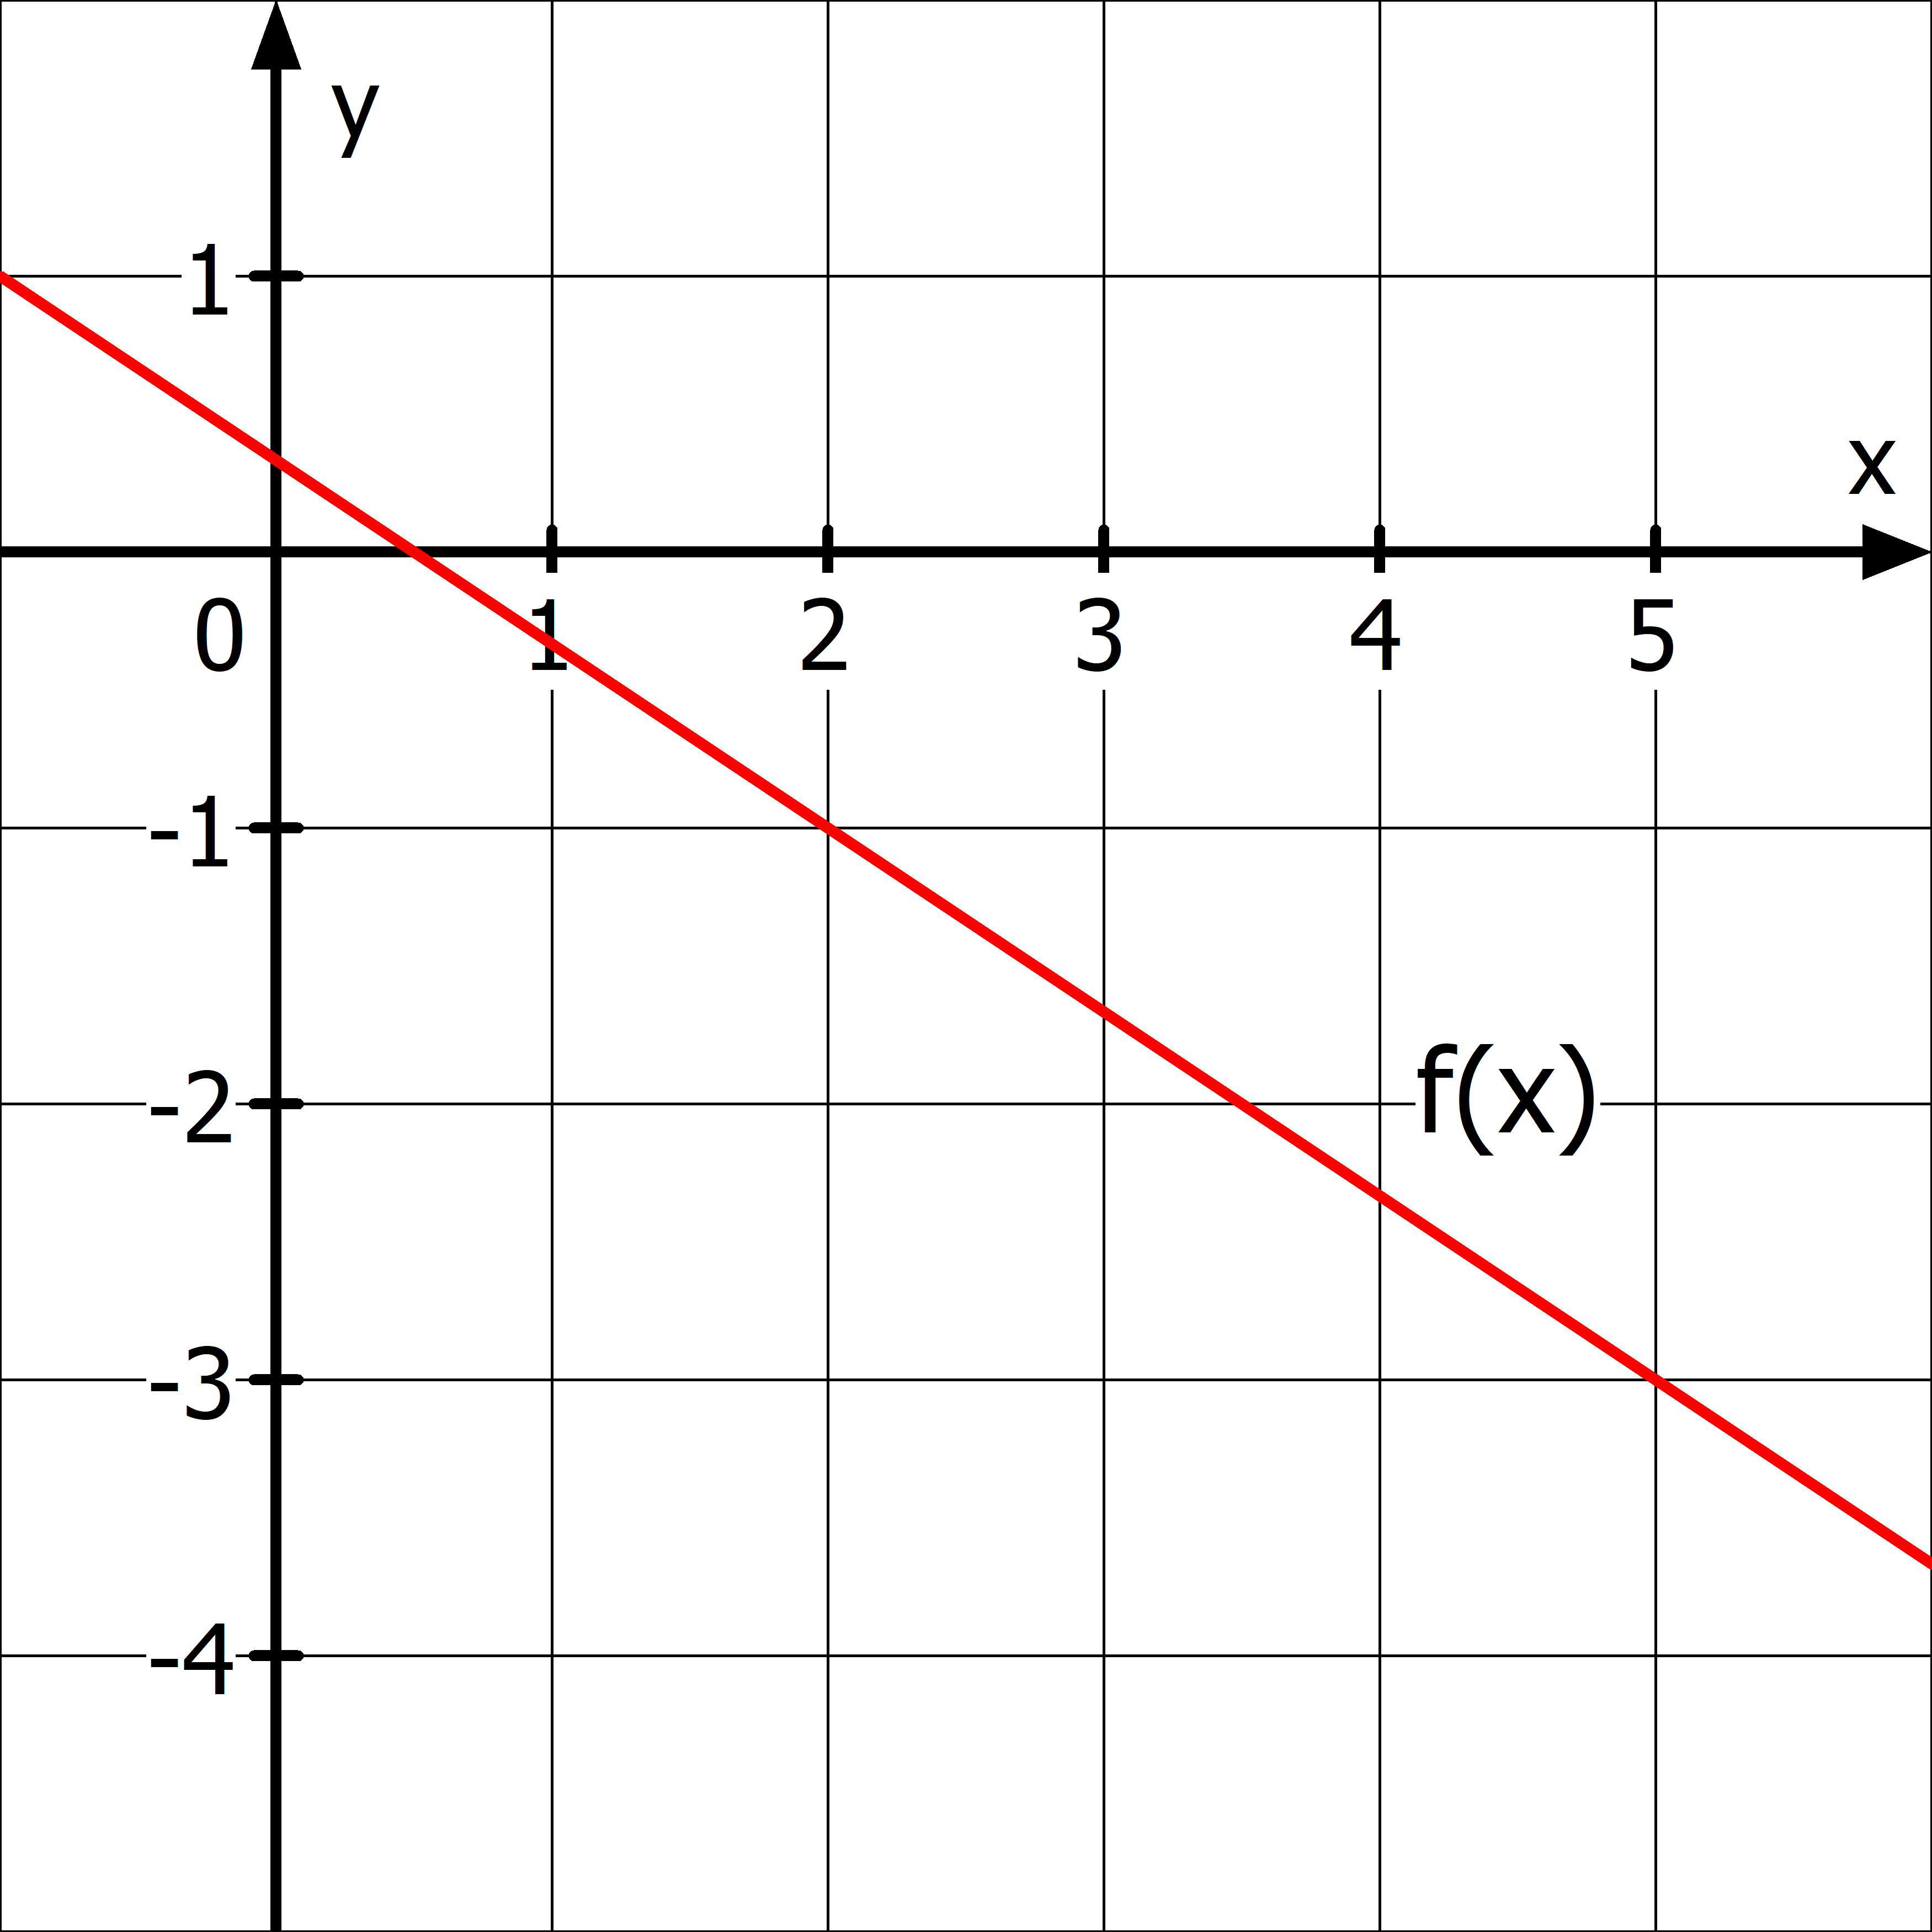
\includegraphics[width=0.90\textwidth]{\linFkt/pics/punktprobe.png}
\end{minipage}}%
\adjustbox{valign=t}{\begin{minipage}{0.5\textwidth}
	Im nebenstehenden Beispiel lässt sich die Steigung der Geraden \(f(x)=mx+b\) leicht über ein Steigungsdreieck bestimmen: \(\textcolor{ForestGreen}{m=-\tfrac{2}{3}}\). Der y-Achsenabschnitt kann leider nicht exakt abgelesen werden. Wir lesen daher einen beliebigen Punkt ab, z.B. \(P(\textcolor{red}{2}\vert\textcolor{blue}{-1})\) und führen mit diesem Punkt eine Punktprobe durch:
	\begin{align*}
		f(\textcolor{red}{2})&=\textcolor{blue}{-1}\\
		\textcolor{loes}{-\dfrac{2}{3}\cdot2+b}&\textcolor{loes}{\;=-1\ \vert+\dfrac{4}{3}}\\
		\textcolor{loes}{b}&\textcolor{loes}{\;=\dfrac{1}{3}}
	\end{align*}

\end{minipage}}%
\end{minipage}
\begin{Exercise}[title={Prüfe, ob die Punkte auf dem Schaubild der Funktion liegen}, label=punktprobeA1]
	\begin{enumerate}[label=\alph*)]
		\item \(f(x)=-x+2\qquad P(2\vert3)\text{ und }Q(-2\vert4)\)
		\item \(g(x)=\dfrac{4}{5}x-1\qquad R(5\vert3)\text{ und }S(10\vert-1)\)
	\end{enumerate}
\end{Exercise}
\begin{Exercise}[title={Bestimme die Funktionsgleichung}, label=punktprobeA2]
	\begin{enumerate}[label=\alph*)]
		\item Das Schaubild der Funktion \(f(x)=2x+b\) verläuft durch den Punkt \(P(2\vert3)\).
		\item Das Schaubild der Funktion \(g(x)=mx-1\) verläuft durch den Punkt \(Q(-2\vert6)\).
		\item Das Schaubild der Funktion \(h(x)=mx+b\) verläuft durch die Punkte \(R_1(2\vert3)\) und \(R_2(4\vert-1)\).
		\item Das Schaubild der Funktion \(i(x)=mx+b\) verläuft durch die Punkte \(S_1(-1\vert-2)\) und \(S_2(5\vert7)\).
	\end{enumerate}
\end{Exercise}
\newpage
\begin{Answer}[ref=punktprobeA1]

	\begin{minipage}{0.5\textwidth}
		\begin{enumerate}[label=\alph*)]
			\item \(f(\textcolor{red}{2})=-\textcolor{red}{2}+2=0\neq\textcolor{blue}{3}\)

			\(P\) liegt nicht auf dem Schaubild von \(f(x)\)

			\(f(\textcolor{red}{-2})=-\left(\textcolor{red}{-2}\right)+2=\textcolor{blue}{4}\)

			\(Q\) liegt auf dem Schaubild von \(f(x)\)
		\end{enumerate}
	\end{minipage}%
	\begin{minipage}{0.5\textwidth}
		\begin{enumerate}[label=\alph*)]
			\setcounter{enumi}{1}
			\item \(g(\textcolor{red}{5})=\tfrac{4}{5}\cdot\textcolor{red}{5}-1=\textcolor{blue}{3}\)

			\(R\) liegt auf dem Schaubild von \(g(x)\)

			\(g(\textcolor{red}{10})=\tfrac{4}{5}\cdot\textcolor{red}{10}-1=7\neq\textcolor{blue}{-1}\)

			\(S\) liegt nicht auf dem Schaubild von \(g(x)\)
		\end{enumerate}
	\end{minipage}%
\end{Answer}
\vspace{1cm}
\begin{Answer}[ref=punktprobeA2]

	\begin{minipage}[t]{0.5\textwidth}
		\begin{enumerate}[label=\alph*)]
			\item Punktprobe mit \(P(\textcolor{red}{2}\vert\textcolor{blue}{3})\)
			\begin{align*}
				f(\textcolor{red}{2})&=\textcolor{blue}{3}\\
				2\cdot\textcolor{red}{2})+b&=\textcolor{blue}{3}\ \vert-4\\
				b&=-1\\
				\Rightarrow f(x)&=2x-1
			\end{align*}
			\item Punktprobe mit \(Q(\textcolor{red}{-2}\vert\textcolor{blue}{6})\)
			\begin{align*}
				g(\textcolor{red}{-2})&=\textcolor{blue}{6}\\
				m\cdot\left(\textcolor{red}{-2}\right)-1&=\textcolor{blue}{6}\ \vert+1\\
				\textcolor{red}{-2}m&=7\ \vert\left(\cdot -\tfrac{1}{2}\right)\\
				m&=-\dfrac{7}{2}\\
				\Rightarrow g(x)&=-\dfrac{7}{2}x-1
			\end{align*}
		\end{enumerate}
	\end{minipage}%
	\begin{minipage}[t]{0.5\textwidth}
		\begin{enumerate}[label=\alph*)]
			\setcounter{enumi}{2}
			\item Bestimmen der Steigung \(m\) mit Hilfe der Punkte \(R_1(\textcolor{red}{2}\vert\textcolor{blue}{3})\) und \(R_2(\textcolor{ForestGreen}{4}\vert\textcolor{YellowOrange}{-1})\):
			\begin{align*}
				m=\dfrac{\textcolor{YellowOrange}{-1}-\textcolor{blue}{3}}{\textcolor{ForestGreen}{4}-\textcolor{red}{2}}=-2
			\end{align*}
			Punktprobe mit \(R_1(\textcolor{red}{2}\vert\textcolor{blue}{3})\) (oder \(R_2\))
			\begin{align*}
				h(\textcolor{red}{2})&=\textcolor{blue}{3}\\
				-2\cdot\textcolor{red}{2}+b&=\textcolor{blue}{3}\ \vert +4\\
				b&=7\\
				\Rightarrow h(x)&=-2x+7
			\end{align*}
			\item Bestimmen der Steigung \(m\) mit Hilfe der Punkte \(S_1(\textcolor{red}{-1}\vert\textcolor{blue}{-2})\) und \(S_2(\textcolor{ForestGreen}{5}\vert\textcolor{YellowOrange}{7})\):
			\begin{align*}
				m=\dfrac{\textcolor{YellowOrange}{7}-\left(\textcolor{blue}{-2}\right)}{\textcolor{ForestGreen}{5}-\left(\textcolor{red}{-1}\right)}=-\dfrac{3}{2}
			\end{align*}
			Punktprobe mit \(S_2(\textcolor{ForestGreen}{5}\vert\textcolor{YellowOrange}{7})\) (oder \(S_1\))
			\begin{align*}
				i(\textcolor{ForestGreen}{5})&=\textcolor{YellowOrange}{7}\\
				\dfrac{3}{2}\cdot\textcolor{ForestGreen}{5}+b&=\textcolor{YellowOrange}{7}\ \vert -\tfrac{15}{2}\\
				b&=-\dfrac{1}{2}\\
				\Rightarrow i(x)&=\dfrac{3}{2}x+-\dfrac{1}{2}
			\end{align*}
		\end{enumerate}
	\end{minipage}%
\end{Answer}